\documentclass{article}
\usepackage{graphicx}
\usepackage[utf8]{ctex}
\usepackage{amsmath}
\usepackage[fontsize=10pt]{fontsize}
\usepackage{geometry}
\geometry{a4paper,left=0.75in,right=0.75in,top=1in,bottom=0.75in}
\usepackage{setspace}
\setlength{\parindent}{0em}
\def\kong{\hspace*{2em}}
\usepackage{amsfonts,amssymb}
\usepackage{xcolor}
\usepackage{fontspec}
\usepackage{enumitem}
\linespread{1.5}
\usepackage{hyperref}
\usepackage{hyperref}
\hypersetup{hidelinks,
	colorlinks=true,
	allcolors=black,
	pdfstartview=Fit,
	breaklinks=true}

\usepackage{listings}
	\lstset{
 columns=fixed,
 numbers=left,
 numberstyle=\tiny\color{gray},
 frame=none,
 backgroundcolor=\color[RGB]{245,245,244},
 keywordstyle=\color[RGB]{40,40,255},
 numberstyle=\footnotesize\color{darkgray},
 commentstyle=\it\color[RGB]{0,96,96},
 stringstyle=\rmfamily\slshape\color[RGB]{128,0,0},
 showstringspaces=false,
 language=c,
 basicstyle=\ttfamily
	}

\usepackage{fancyhdr}

\pagestyle{fancy}
\fancyhf{}
\fancyhead[LE,RO]{\thepage}
\fancyhead[RE,LO]{\kaishu PB21000276施耀炜}



\date{2022年3月}

\begin{document}

\setcounter{page}{1}
\thispagestyle{empty}
\kong
\\[10pt]
\begin{center}
	\textbf{\huge \heiti 实验报告五}\\[6pt]
    \textbf{\huge \heiti 整流滤波电路及应用}\\[12pt]
	\textbf{学号：}\underline{\kaishu PB21000276} \qquad 
    \textbf{姓名：}\underline{\kaishu 施耀炜} \qquad 
    \textbf{班级：}\underline{\kaishu 21级少院6班}\qquad 
    \textbf{日期：}\underline{2022年5月4日}\\[24pt]
\end{center}
\section{实验名称}
    \kong 整流滤波电路及应用
\section{实验目的}
    \kong 了解交流信号的几个参数，学习整流滤波电路的基本工作原理及制作一台直流电源。
\section{实验原理}
    \kong 整流电路的作用是把交流电转换成直流电，严格地讲是单方向大脉动直流电，
    而滤波电路的作用是把大脉动直流电处理成平滑的脉动小的直流电。
    \subsection{整流原理}
        \kong 利用二极管的单向导电性可实现整流。\\
        \kong (1)半波整流：利用单个二极管，交流电中和二极管导通方向相同的部分可以显示出来，如图5.1。\\
        \kong (2)全波整流：利用四个二极管组成的桥式等结构，使交流电变的正负半周期信号都被应用，如图5.2。\\[18pt]
        \begin{minipage}{0.5\linewidth}
            \centering
            \textbf{图\ 5.1}\quad 半波整流电路及其波形图  \\[4pt]
            
\includegraphics[width=0.9\linewidth]{tp1.png}
            \label{tp1.png} 
        \end{minipage}
        %\qquad
        \begin{minipage}{0.5\linewidth}
            \centering
            \textbf{图\ 5.2}\quad 桥式全波整流电路及其波形图 \\[4pt]
            
\includegraphics[width=0.9\linewidth]{tp2.png}
            \label{tp2.png}
        \end{minipage}
    \subsection{滤波原理}
        \kong 经过整流后的电压(电流)仍然是有“脉动”的直流电，为了减少被波动，通常要加滤波器，
        常用的滤波电路有电容、电感滤波等。本实验使用电容滤波。\\
        \kong (1)单电容滤波：利用一个电容与负载并联，作为滤波，如图5.3。\\
        \kong (2)$\pi$型电容滤波：即在单电容滤波基础上，在此之后又加了一级RC滤波，如图5.4。\\
        \begin{minipage}{0.5\linewidth}
            \centering
            \textbf{图\ 5.3}\quad 单电容滤波电路  \\[4pt]
            
\includegraphics[width=0.9\linewidth]{tp3.png}
            \label{tp3.png} 
        \end{minipage}
        %\qquad
        \begin{minipage}{0.5\linewidth}
            \centering
            \textbf{图\ 5.4}\quad $\pi$型电容滤波电路 \\[4pt]
            
\includegraphics[width=0.9\linewidth]{tp4.png}
            \label{tp4.png}
        \end{minipage}\\
        \kong 纹波系数是指负载上交流电压的有效值与直流电压之比，是表征直流电源品质的一个重要参数。
        除了与整流滤波电路品质有关之外，与外电路负载关系也很大。即：
        $$
            K_u=\frac{\text{交流电压有效值}}{\text{直流电源}}\times 100\% \eqno{(5.1)}
        $$
    
%实验仪器
\section{实验仪器}
    \begin{itemize}[noitemsep]
        \item 信号发生器
        \item 数字电压表（直流电压档、交流电压档）
        \item 电阻箱
        \item 面包板（整流二极管、电容、电阻）
        \item 导线
    \end{itemize}
%数据处理与分析
\newpage
\section{实验数据与处理、分析}
    \subsection{整流、滤波电路}
        \subsubsection{整流电路}
        \kong 如图5.5，5.6，5.7所示，分别为初始信号、半波整流后的信号、全波整流后的信号的波形图。\\[14pt]
        \begin{minipage}{0.33\linewidth}
            \centering
            \textbf{图\ 5.5}\quad 初始信号波形图 \\[4pt]
            
\includegraphics[width=0.9\linewidth]{tp5.jpg}
            \label{tp5.png} 
        \end{minipage}
        \begin{minipage}{0.33\linewidth}
            \centering
            \textbf{图\ 5.6}\quad 半波整流波形图 \\[4pt]
            
\includegraphics[width=0.9\linewidth]{tp6.jpg}
            \label{tp6.png}
        \end{minipage}
        \begin{minipage}{0.33\linewidth}
            \centering
            \textbf{图\ 5.7}\quad 全波整流波形图 \\[4pt]
            
\includegraphics[width=0.9\linewidth]{tp7.jpg}
            \label{tp7.png}
        \end{minipage}
        \subsubsection{滤波电路}
        \kong 如图5.8，5.9所示，分别为全波整流后的电流经过单电容($1\mu F$)滤波、$\pi$型电容($1\mu F\times 2$)滤波后的波形图。\\[14pt]
        \begin{minipage}{0.5\linewidth}
            \centering
            \textbf{图\ 5.8}\quad 单电容($1\mu F$)滤波波形图 \\[4pt]
            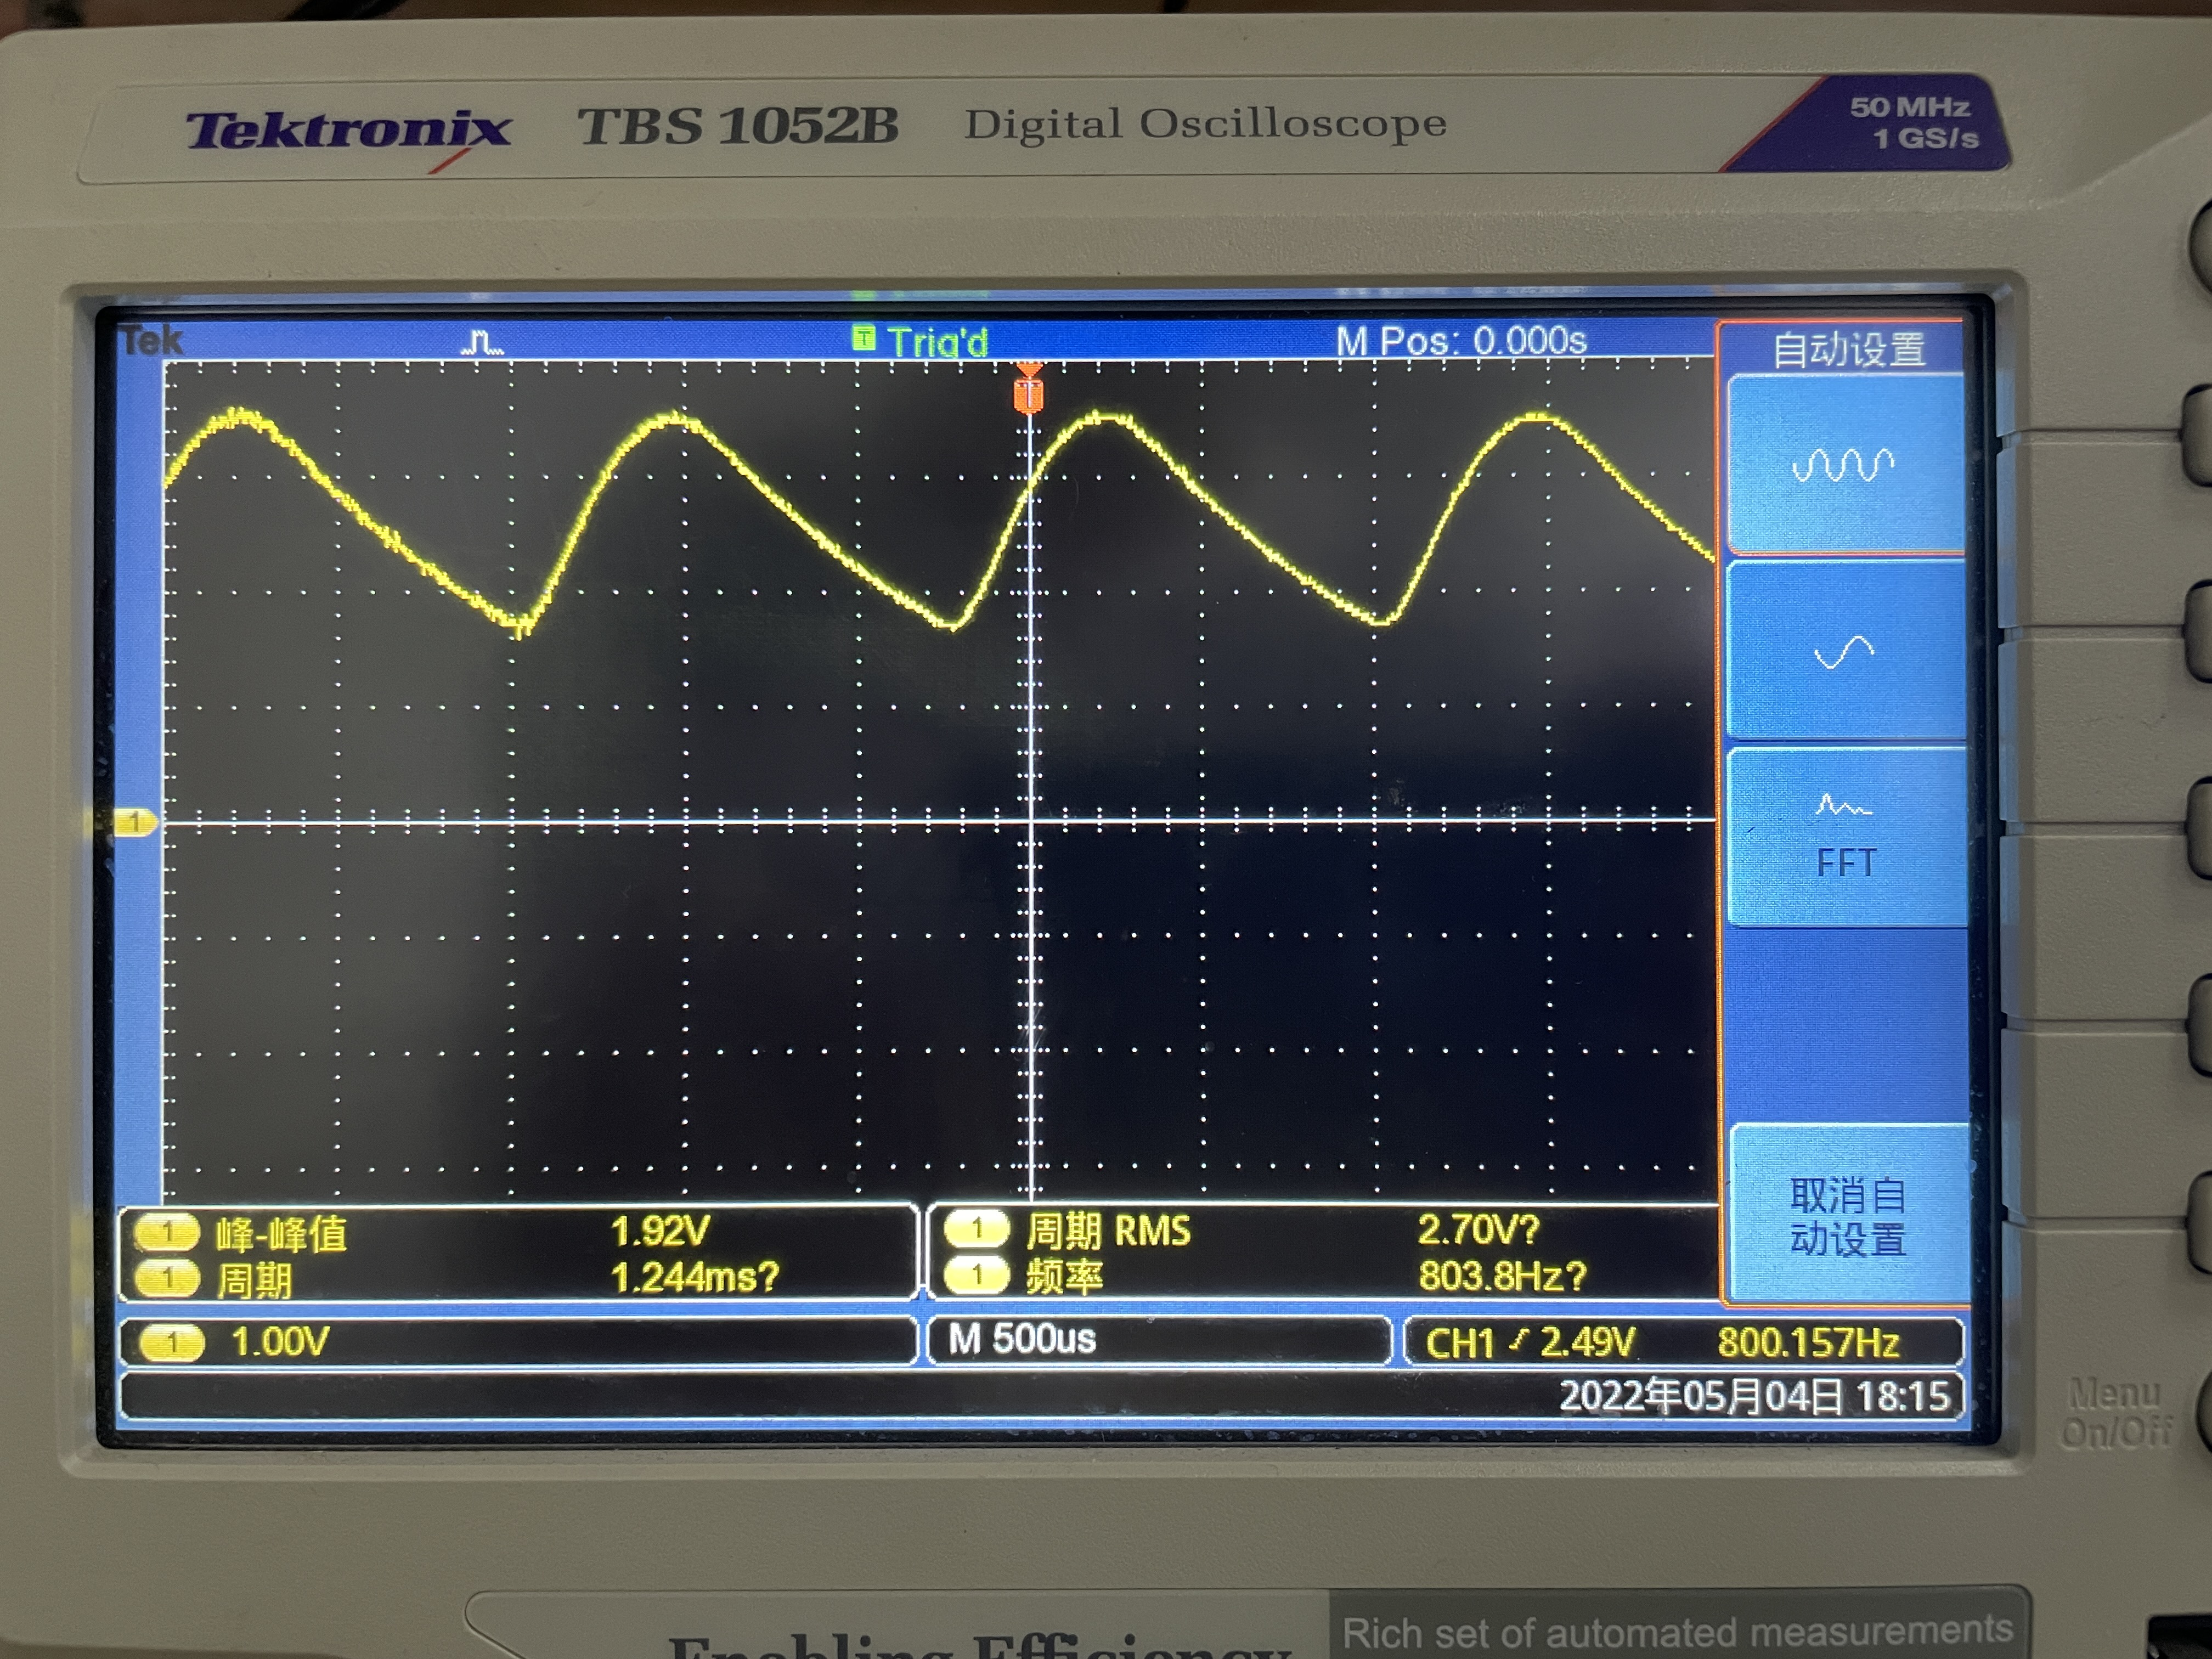
\includegraphics[width=0.9\linewidth]{tp8.jpg}
            \label{tp8.png}
        \end{minipage}
        \begin{minipage}{0.5\linewidth}
            \centering
            \textbf{图\ 5.9}\quad $\pi$型电容($1\mu F\times 2$)滤波波形图 \\[4pt]
            \includegraphics[width=0.9\linewidth]{tp9.jpg}
            \label{tp9.png}
        \end{minipage}\\[14pt]
        \kong 下表5.1为滤波后的直流电压和交流电压有效值，以及计算得到的纹波系数。
        \begin{center}
            \textbf{表\ 5.1}\quad $1\mu F$电容滤波数据  \\[4pt]
            \begin{tabular}{|c|c|c|c|}
            \hline
                    滤波种类        & 直流电压/$V$   & 交流电压有效值/$V$  & 纹波系数  \\ \hline
                    单电容滤波      & 2.585         & 0.5795            & 22.416\% \\ \hline
                    $\pi$型电容滤波 & 1.4859        & 0.0650            & 4.374\% \\ \hline
            \end{tabular}
        \end{center}
    \subsection{电容对滤波效果的影响}
        \kong 将上述所有$1\mu F$更改为$10\mu F$，重新测量直流电压和交流电压有效值，再计算纹波系数，
        波形如下图5.10，5.11，数据如下表5.2。\\[14pt]
        \begin{minipage}{0.5\linewidth}
            \centering
            \textbf{图\ 5.10}\quad 单电容($10\mu F$)滤波波形图 \\[4pt]
            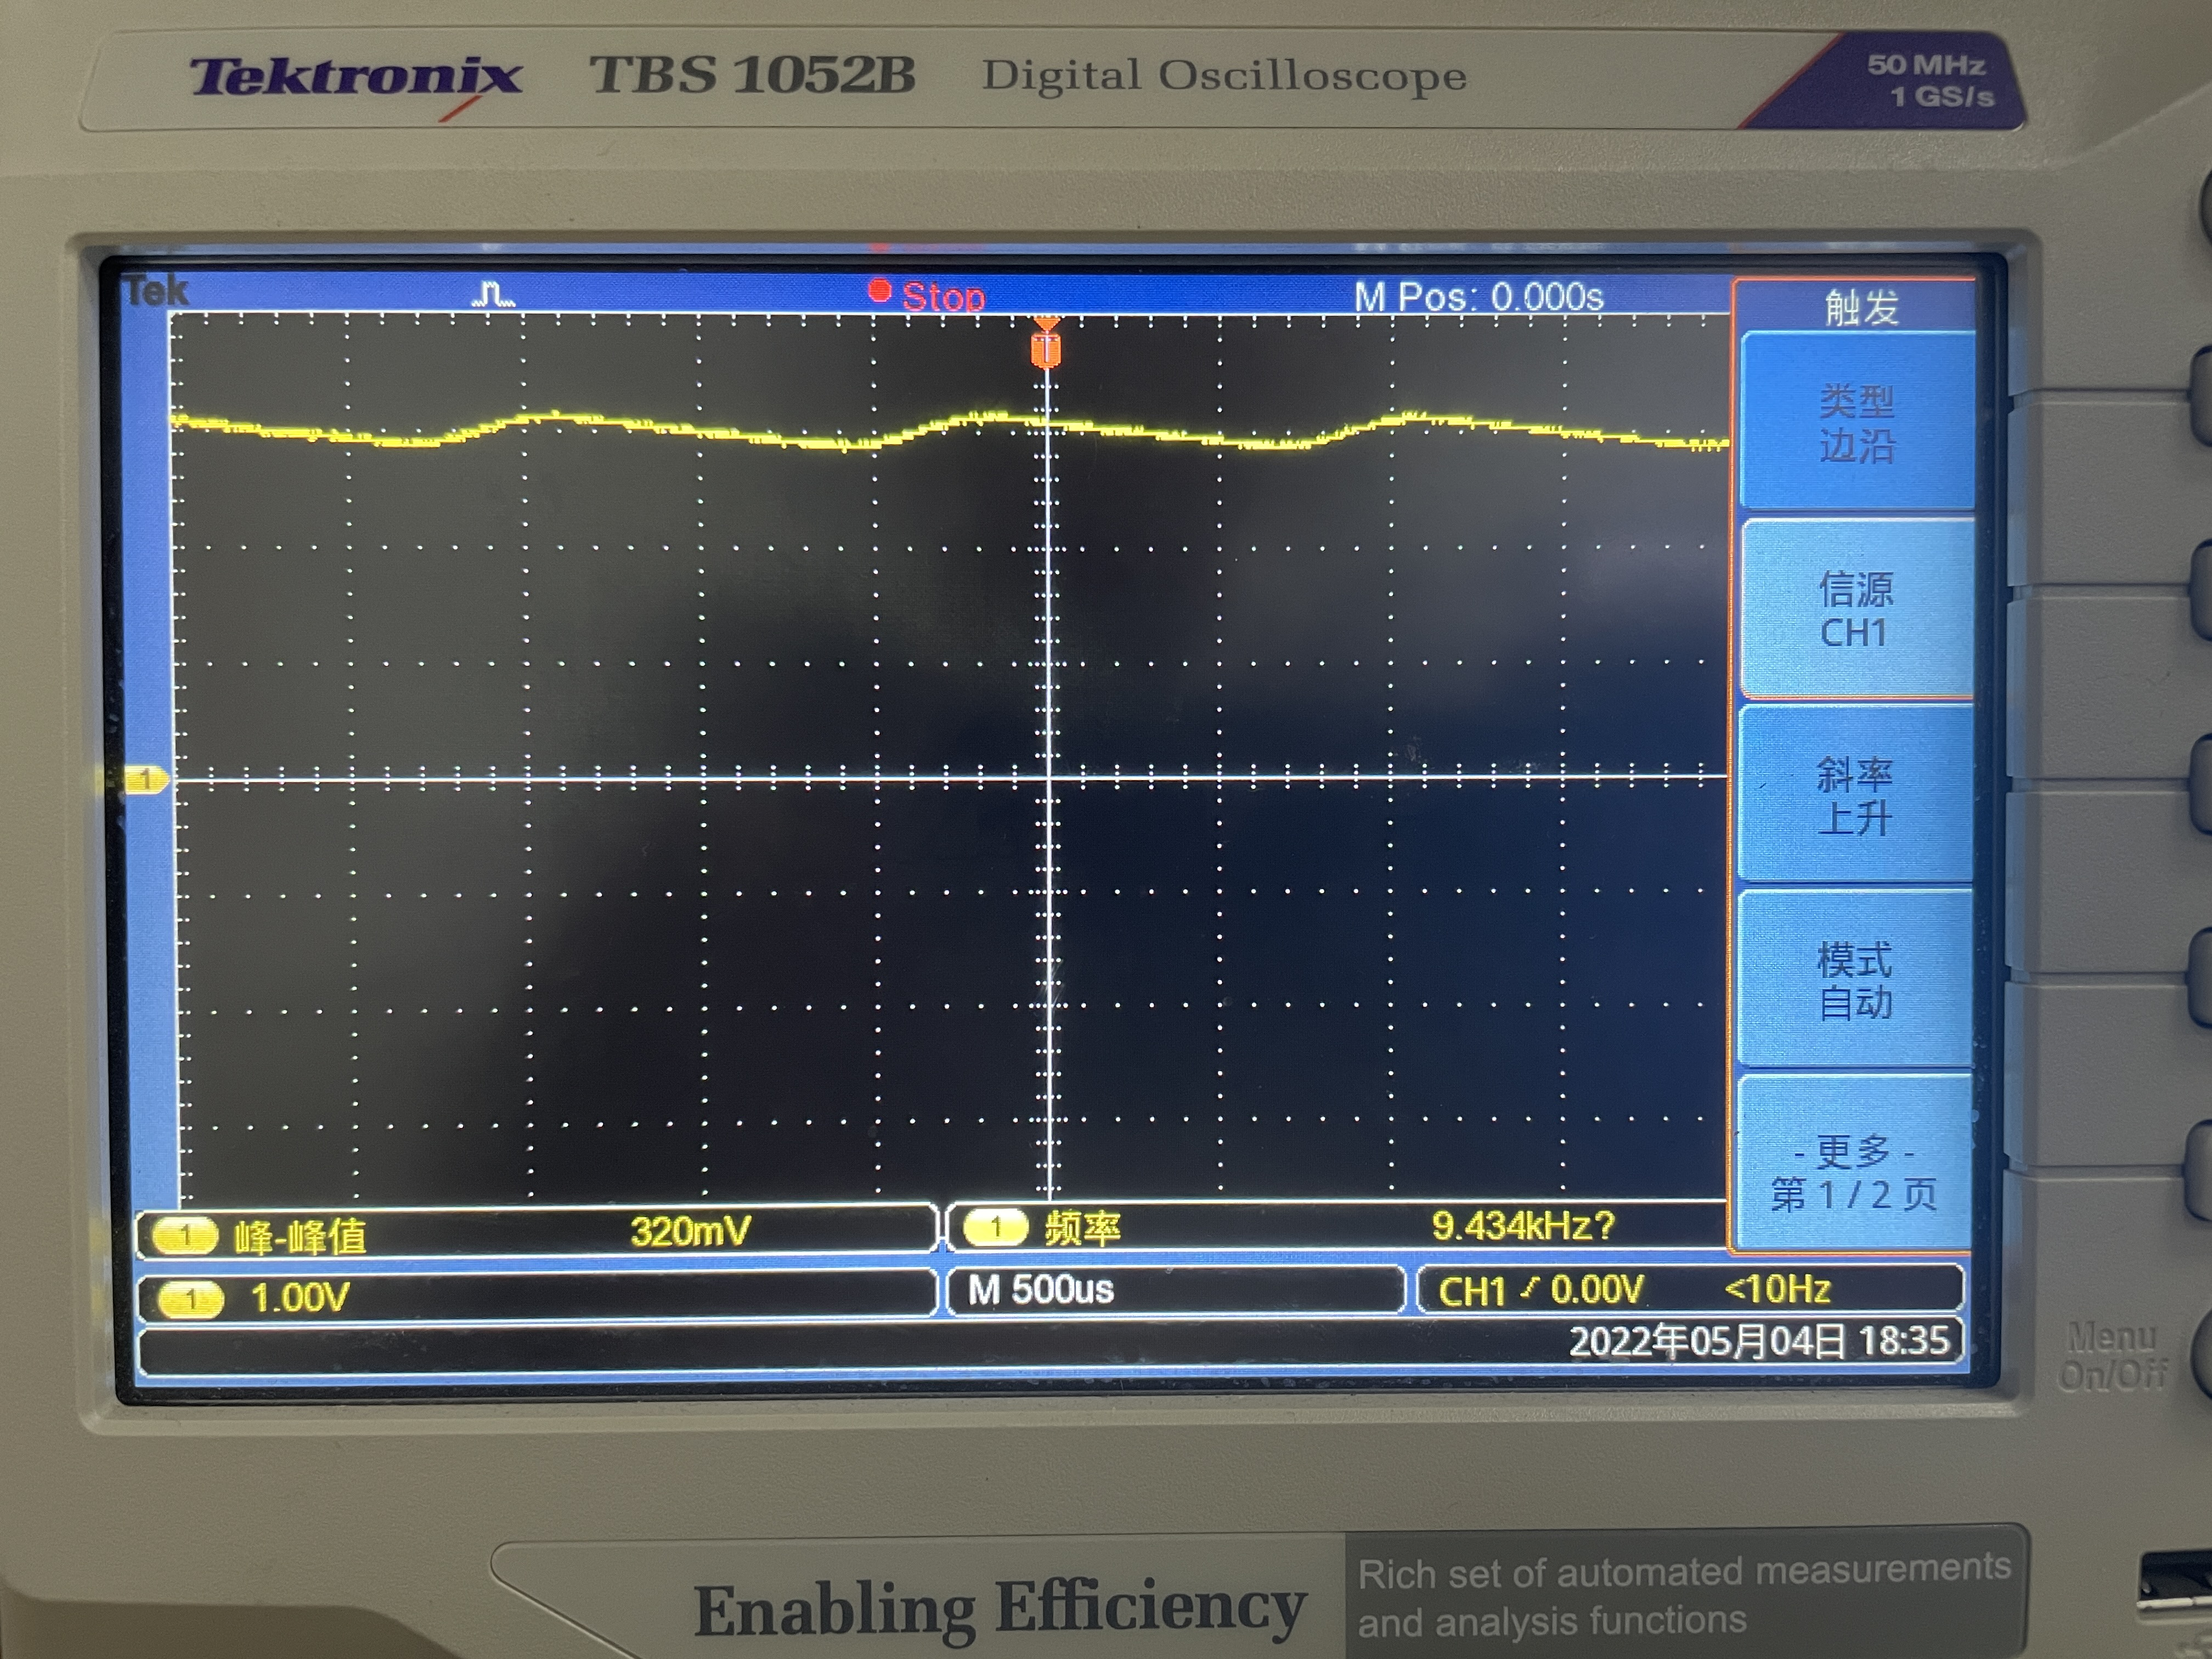
\includegraphics[width=0.9\linewidth]{tp11.jpg}
            \label{tp10.png}
        \end{minipage}
        \begin{minipage}{0.5\linewidth}
            \centering
            \textbf{图\ 5.11}\quad $\pi$型电容($10\mu F\times 2$)滤波波形图 \\[4pt]
            \includegraphics[width=0.9\linewidth]{tp10.jpg}
            \label{tp11.png}
        \end{minipage}
        \begin{center}
            \textbf{表\ 5.1}\quad $10\mu F$电容滤波数据  \\[4pt]
            \begin{tabular}{|c|c|c|c|}
            \hline
                    滤波种类        & 直流电压/$V$   & 交流电压有效值/$V$  & 纹波系数  \\ \hline
                    单电容滤波      & 2.954         & 0.0745            & 2.522\% \\ \hline
                    $\pi$型电容滤波 & 1.6089        & 0.00000           & 0.000\% \\ \hline
            \end{tabular}
        \end{center}
        \kong 和原实验相比，电容增大，电容充放电能力、蓄电能力增强，则对于电路的交流部分削弱的更明显，
        即交流部分更小，同时直流部分也有所增加，纹波系数也更小。
    \subsection{信号源频率对滤波效果的影响}
        \kong 固定电容 1$\mu F$，整流滤波电路，改变信号源频率从 $10\sim2000Hz$，
        测量直流电压和交流电压有效值，并计算对应频率下的纹波系数，如下表5.3，5.4。\\[14pt]
        \begin{minipage}{1\linewidth}
            \centering
            \textbf{表\ 5.3}\quad 单电容在不同频率下的滤波数据  \\[4pt]
            \begin{tabular}{|c|c|c|c|}
            \hline
                    频率/$Hz$        & 直流电压/$V$   & 交流电压有效值/$V$  & 纹波系数  \\ \hline
                    10   & 1.968 & 1.2497 & 63.501\% \\ \hline
                    20   & 1.978 & 1.2364 & 62.508\% \\ \hline
                    30   & 1.991 & 1.1286 & 56.685\% \\ \hline
                    50   & 2.024 & 1.1743 & 58.019\% \\ \hline
                    100  & 2.127 & 1.0518 & 49.450\% \\ \hline
                    200  & 2.326 & 0.8407 & 36.144\% \\ \hline
                    400  & 2.585 & 0.5795 & 22.418\% \\ \hline
                    600  & 2.715 & 0.4296 & 15.823\% \\ \hline
                    1000 & 2.828 & 0.2609 & 6.598\% \\ \hline
                    1500 & 2.884 & 0.1412 & 4.896\% \\ \hline
                    2000 & 2.899 & 0.0621 & 2.142\% \\ \hline
            \end{tabular}\\[14pt]
        \end{minipage}\\[14pt]
        \begin{minipage}{1\linewidth}
            \centering
            \textbf{表\ 5.4}\quad $\pi$型电容在不同频率下的滤波数据  \\[4pt]
            \begin{tabular}{|c|c|c|c|}
            \hline
                    频率/$Hz$        & 直流电压/$V$   & 交流电压有效值/$V$  & 纹波系数  \\ \hline
                    10   & 1.0390 & 0.6333 & 60.953\% \\ \hline
                    20   & 1.0603 & 0.6009 & 57.521\% \\ \hline
                    30   & 1.0862 & 0.5633 & 51.860\% \\ \hline
                    50   & 1.1403 & 0.4866 & 42.573\% \\ \hline
                    100  & 1.2522 & 0.3320 & 26.513\% \\ \hline
                    200  & 1.3751 & 0.1706 & 12.406\% \\ \hline
                    400  & 1.4859 & 0.0650 & 4.377\% \\ \hline
                    600  & 1.5331 & 0.0326 & 2.126\% \\ \hline
                    1000 & 1.5701 & 0.0118 & 0.752\% \\ \hline
                    1500 & 1.5851 & 0.0032 & 0.202\% \\ \hline
                    2000 & 1.5908 & 0.0000 & 0.000\% \\ \hline
            \end{tabular}
        \end{minipage}\\[14pt]
        \kong 随着频率的上升，直流电压逐步上升，而交流电压和纹波系数下降。
        同时，同频率下$\pi$型电路的纹波系数始终低于单电容电路，但其输出电压也始终较低。
        两种电路均有信号源的频率越高，纹波系数越低的特点，而$\pi$型电路随频率的升高，纹波系数下降更快。
    
\section{思考题}
    \kong \textbf{1.}整流、滤波的主要目的是什么?\\
    \kong \textbf{答：}把交流电源改为直流电源。可以使电流更加的稳定，供一般的电路使用。\\
    \kong \textbf{2.}滤波电路中电容是否越大越好？请根据实验过程简述理由。\\
    \kong \textbf{答：}不是，虽然理想的状态下可以认为电容越大会使纹波系数更小，
    但是实际实验中当电容变大时，电压会减小，产生大量的浪费使得电路可用性变低。\\
\end{document}
